\chapter{Methodology}

\section{Data Generation Pipeline}
\label{sec:datagen:method}
\begin{figure}[htbp]
	\centering
	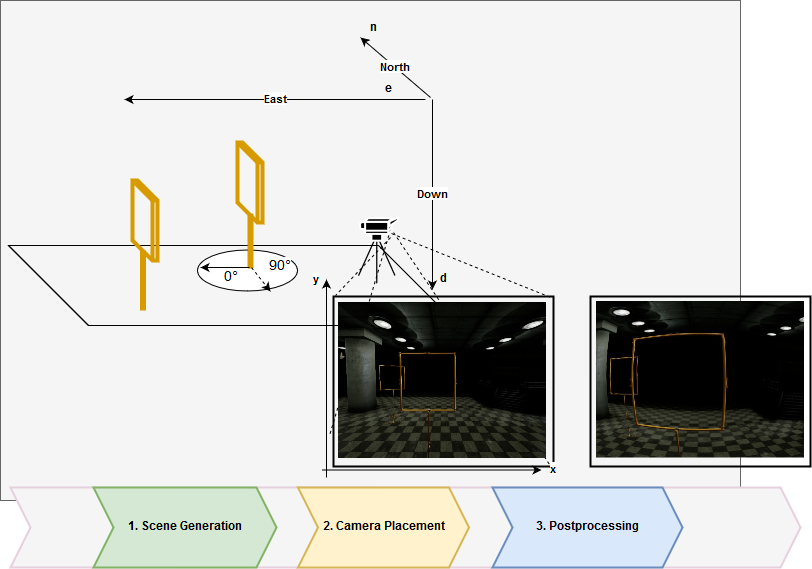
\includegraphics[width=0.9\textwidth]{fig/datagen_notation}
	\caption{Overview of the data generation process.}
	\label{fig:training:datagen_notation}
\end{figure}

A data generation pipeline is implemented using OpenGL, UnrealEngine and AirSim. An overview can be seen in \Cref{fig:training:datagen_notation}. In the first step a scene is created in which the objects of interest as well as the camera are placed. In 3D space position and orientation (pose) of each object are determined by translation $\textbf{t}$ and rotation $\textbf{r}$. The coordinate system is \ac{NED}.

A view projection yields an image through the lens of the camera. The coordinates of each point in 3D space are projected on the 2D image plane. A final post processing step can simulate further effects like lens distortion and sensor noise. This step is implemented using OpenCV and Python. All source code is made publicly available at \url{https://github.com/phildue/datagen.git}.

\subsection{Environments}

Within the pipeline environments for training and testing are created. A black environment serves as base to replace the background with existing images. Furthermore, three indoor base environments are created that fully simulate illumination and background. An overview can be seen in \Cref{fig:environments}. Within the environment light conditions, background textures, object locations can be changed manually. The environments are described in the following:

\begin{enumerate}
	\item \textit{Dark:} The environment is a room without windows, only containing artificial light sources. 
	\item \textit{Daylight:} The environment is a room with windows along all walls that allow daylight to illuminate the room. The windows can lead to strong variations in the contrast between different parts of the object.
	\item \textit{IROS:} The environment resembles the room of the \ac{IROS} Autonomous Drone Race 2018. The light sources stem from a window front at one side of the room, as well as artificial light sources at the ceiling. Depending on the view point, the object might appear against bright or dark background.
\end{enumerate}

\begin{figure}[hbtp]
	\centering
	\begin{minipage}{0.3\textwidth}
		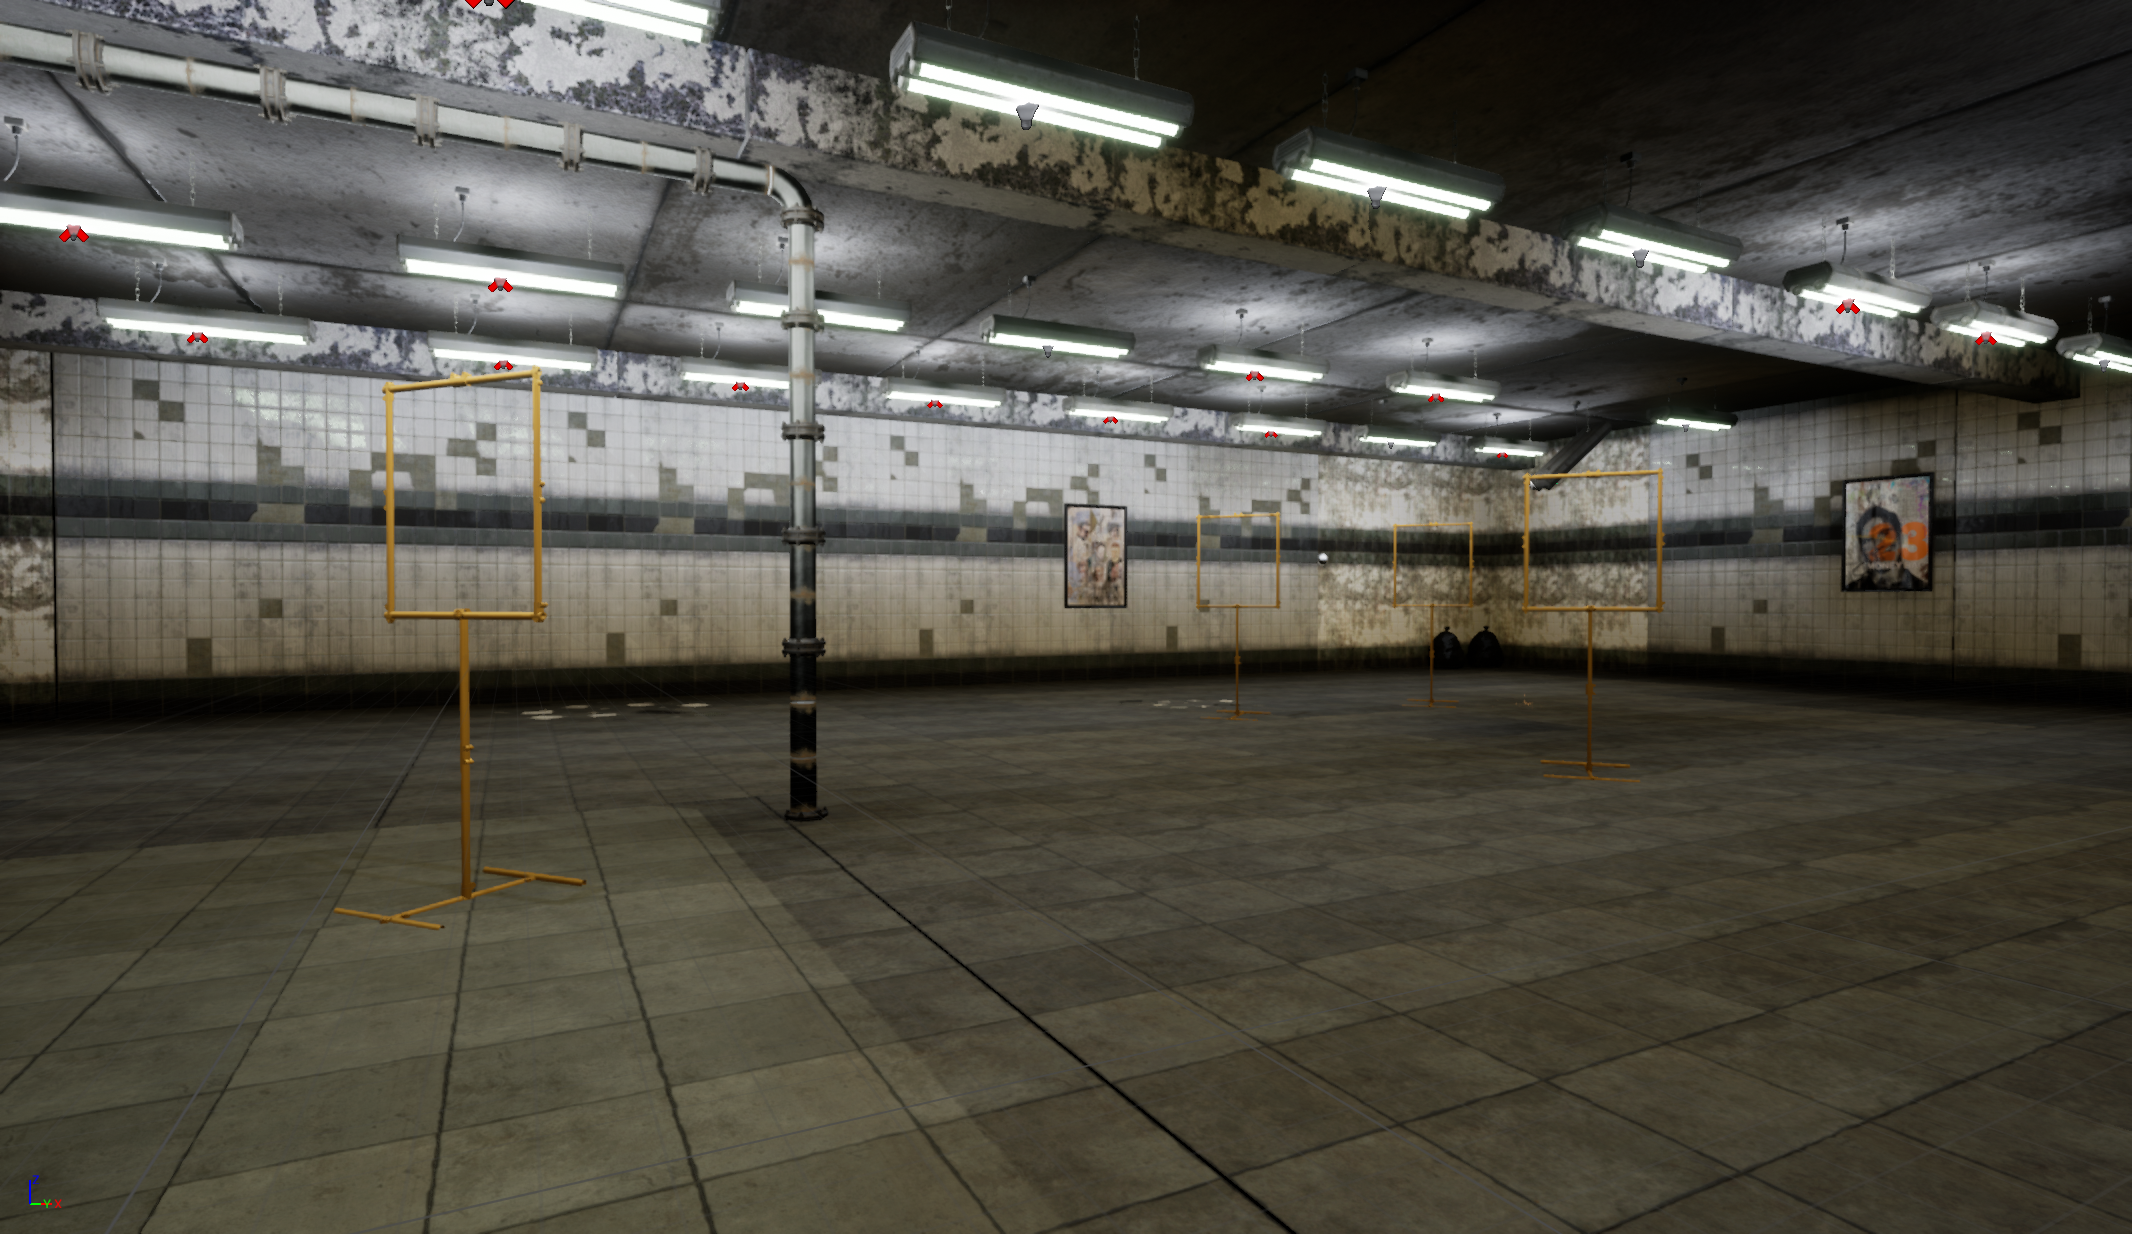
\includegraphics[width=\textwidth]{fig/basement_perspective}
	\end{minipage}
	\begin{minipage}{0.3\textwidth}
		\includegraphics[width=\textwidth]{fig/daylight_perspective}
	\end{minipage}
	\begin{minipage}{0.3\textwidth}
		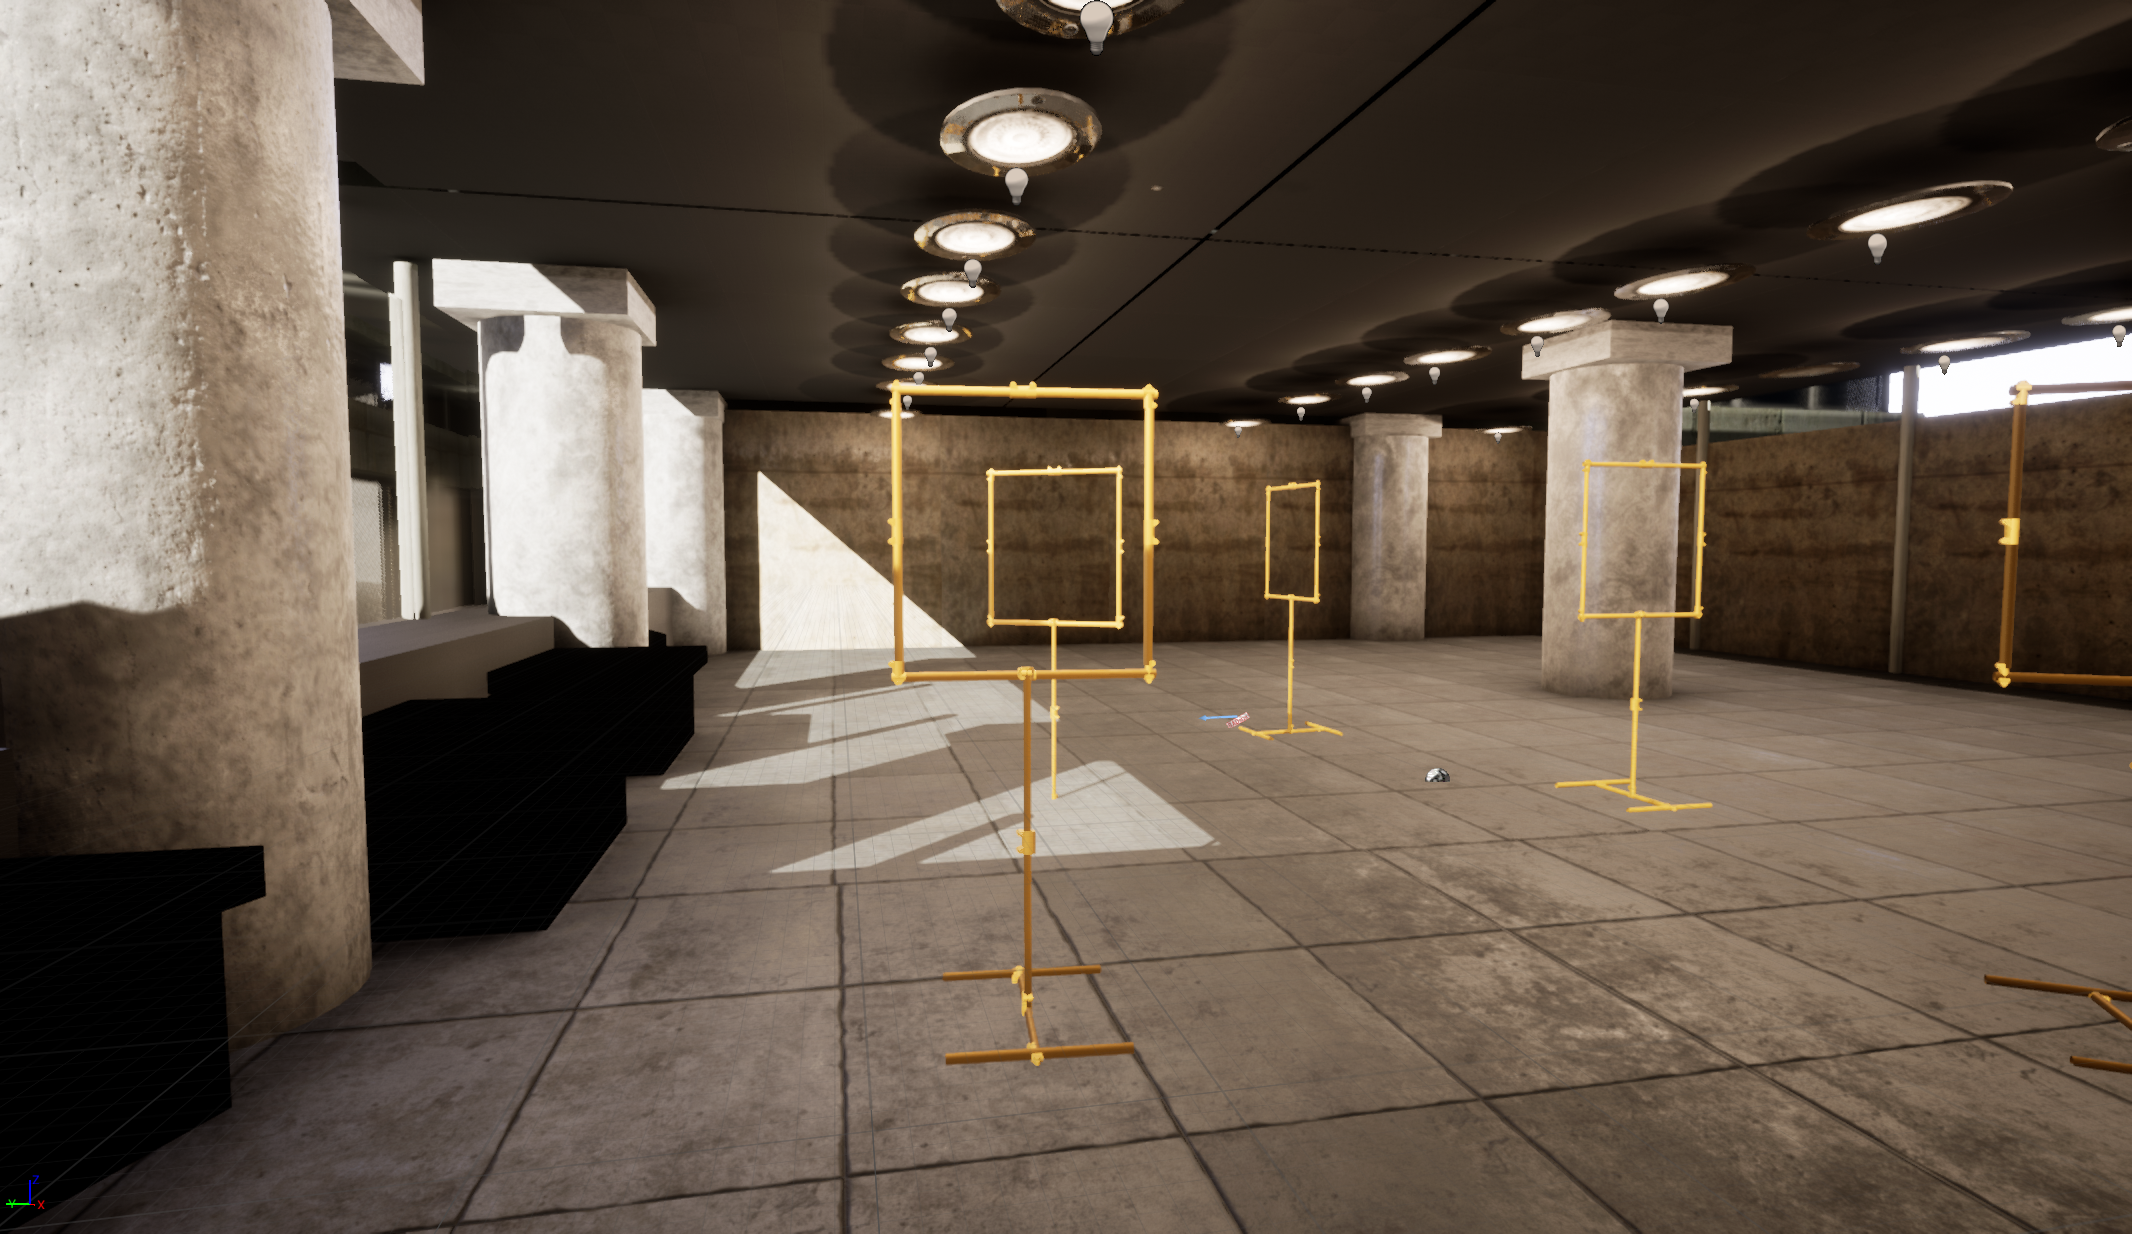
\includegraphics[width=\textwidth]{fig/iros_perspective}
	\end{minipage}
	\caption{The environments from left to right \textit{Dark}, \textit{Daylight}, \textit{IROS2018}}
	\label{fig:environments}
\end{figure}

The data generation pipeline is used to generate a test set in simulation. The test set is set up in the \textit{IROS} environment and inspired by the race court of the \ac{IROS} Autonomous Drone Race. The AirSim flight controller is used to simulate a flight of an \ac{MAV} through the race court. The test set contains 550 images with a total of 1361\todo{recount with filtered} objects.

It should be noted that when generating data with the described methods it is likely that samples appear in which only a corner of the object is visible or the view angle is in such a way that the object appears only as a thin line. In initial experiments these corner cases led to unstable training. Hence, some minimum requirements for the labels are set and samples/labels are removed if these are not met. Objects have to have a minimum size of 1\% of the image area as well as an aspect ratio between 1/3 and 3/1. Furthermore, at least three corners have to be visible.

The models and training are implemented using the \textit{Keras} framework with \textit{tensorflow}-backend. For all trainings the Adam optimizer is applied using a learning rate of 0.001 for the first 60 epochs and a learning rate 0.0001 afterwards. A validation set containing 1\% randomly sampled images from the training set is used. The training is stopped if the validation error does not decrease for more than 5 epochs or 100 epochs are reached.

Throughout the experiments the baseline TinyYoloV3 architecture is used. Thereby we simplify the loss function to a single class prediction. The exact model is described in \Cref{sec:object_detection}. The input image resolution is 416x416.

\subsection{Image Augmentation}

The final step applies low-level image transformations. It allows to further simulate sensor effects and increase the variance in the generated data.

In literature \cite{Krizhevsky2012a,Howard2013,Redmon,Liu} the application of image augmentation is a common tool to improve the detection performance. The experiments in \cite{Carlson2018} show how the incorporation of sensor effects particularly improves the performance of models learned on fully synthesized data. In the \ac{MAV} domain sensor and lens effects have a significant influence on the obtained sample. Hence, we hypothesize that the incorporation of these effects will improve the performance of the trained models. A total of  five image augmentation techniques are investigated.

\paragraph{Lens Distortion}

Lens distortion is a form of optical aberration which causes light to not fall in a single point but a region of space. For \acp{MAV} commonly used wide-angle lenses, this leads to barrel distortion and thus to straight lines appearing as curves in the image.

For this work a 120 wide angle lens is used. Especially, close objects undergo a strong variation in appearance. Hence, we hypothesize including this effect in the training process will improve the performance on the real world dataset. 

The effect is applied using the model for wide-angle lenses from \cite{Vass}. It models the removal of lens distortion as combination of radial and non-radial part, that is approximated with a second order Taylor expansion:
\todo{double check formula is (y in first line?)}
\begin{equation}
\begin{pmatrix}
x_u \\
y_u  
\end{pmatrix}=
f(x,y) =
\begin{pmatrix}
x (1 + \kappa_1 x^2 + \kappa_1 (1 + \lambda_x) y^2 + \kappa_2(x^2 + y^2)^2) \\
y (1 + \kappa_1 x^2 + \kappa_1 (1 + \lambda_y) y^2 + \kappa_2(x^2 + y^2)^2)
\end{pmatrix} 
\label{eq:distortion}
\end{equation}
Where:
\begin{itemize}
	\item $x_u$ and $y_u$ are the undistorted coordinates.
	\item $\kappa_1$ $\kappa_2$ control the radial distortion 
	\item $\lambda_x$ and $\lambda_y$ control the tangential distortion
\end{itemize}

Applying the lens distortion to an image is done using the inverse of \Cref{eq:distortion}. However, as there is no closed form solution, so the Newton-approximation.

An example with $\kappa_1 = 0.5, \kappa_2 = 0.5$ is displayed in \Cref{fig:distortion}. It can be seen how the previously straight lines appear as circular shape.

\paragraph{Chromatic Aberration.}

Chromatic Aberration is caused when different wavelengths of light do not end up in the same locations of the visual sensor. This leads to a shift in the colour channels of the image.

In \cite{Carlson2018} including chromatic aberration significantly improves the performance of models that are trained on fully synthesized data. Hence, we hypothesizes this will also help for our work.

Similarly to \cite{Carlson2018}, chromatic aberration is applied by scaling the locations of the green channel, as well as applying translations on all channels. The model can be implemented as affine transformation of the pixel locations for each channel:

\begin{equation}
f(x_C,y_C) = \begin{pmatrix}
S & 0 & t_x \\
0 & S & t_y \\
0 & 0 & 1
\end{pmatrix} \begin{pmatrix}
x_C \\
y_C \\
1
\end{pmatrix}
\end{equation}

Where $C$ is one colour channel of the image.

An example is displayed in \Cref{fig:chromatic}. It can be seen how the red and green channel are shifted relative to each other. Thus two bars appear in the image.

\paragraph{Blur}

Fast movement and sensor noise can lead to blurry images. This is particularly present in the domain of \ac{MAV}/Autonomous Drone Racing. Hence, we hypothesize including this effect will improve the detection in the real world. 

The effect is modelled using a Gaussian-filter. The image is convolved with a 2D-kernel build from:

\begin{equation}
k(x,y) = \frac{1}{2\sigma_x\sigma_y\pi}e^{-\frac{1}{2}({\frac{(x-\mu_x)^2}{\sigma_x^2} + \frac{(y-\mu_y)^2}{\sigma_y^2}})}
\end{equation}

Where $\sigma_x$ and $\sigma_y$ are the variance in direction x and y, used to model directional (motion) blur and $\mu_x$, $\mu_y$ are at the kernel center. An example can be seen in \Cref{fig:focusblur}.

\paragraph{Exposure.}

Exposure is the time the sensor records light in order to create an image. Over- and Underexposure are caused when this time is too short or too long, leading to too dark or too bright images.

Cameras typically have Autoexposure-functionality which adapts the exposure time depending on light conditions. However, the adoption is not instant, sudden light changes can lead to over- or underexposure. This particularly applies during a fast flight. Hence, we hypothesize incorporating the effect in the data generation will improve the performance of the trained model. The effect is modelled following \cite{Carlson2018}:

\begin{equation}
f(S) = \frac{255}{1 + e^{-A S}}
\end{equation}
where $A$ is a constant term for contrast and $S$ the exposure.
\todo{whats a}
The image can be re-exposed with:

\begin{equation}
I' = f(S+\Delta S)
\end{equation}

where $S$ is obtained from :
\begin{equation}
S = f^{-1}(I)
\end{equation}

An example for overexposure is displayed in \Cref{fig:exposure}. It can be seen how lighter areas appear particularly light, while dark areas remain dark.

\paragraph{Colour Variations}

The 3D-models and textures used in the simulator are limited and creating a large variation in environments or objects requires manual effort. An alternative method to increase the variation in colour and illumination is a scaling in HSV space. The objects in the real world dataset have a slightly different shape and different colour to the 3D-models of the data generation tool. We hypothesize including variations in HSV space will improve the performance on the real world dataset.

The variations are including with:
\begin{equation}
I^* = f(I) = S I
\end{equation}
Where \textbf{S} is a 3D-vector where each element stems from a uniform distribution. The distributions are:


\begin{figure}[htbp]
	\centering
	\begin{minipage}{0.33\textwidth}
		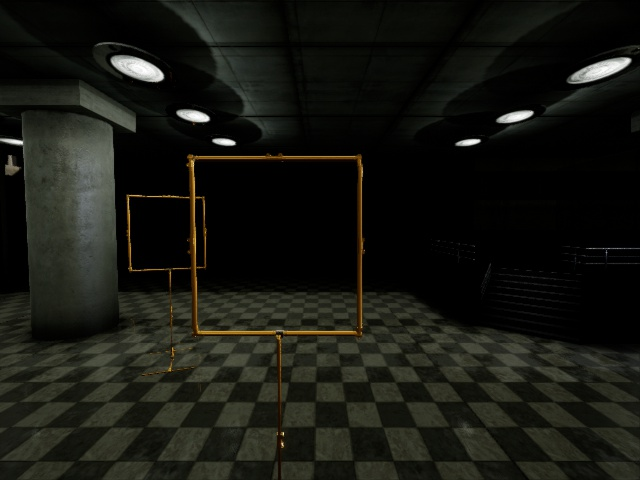
\includegraphics[width=\textwidth]{fig/gate_example}
		\caption{Original Image.}
		\label{fig:orig}
	\end{minipage}
	\begin{minipage}{0.33\textwidth}
		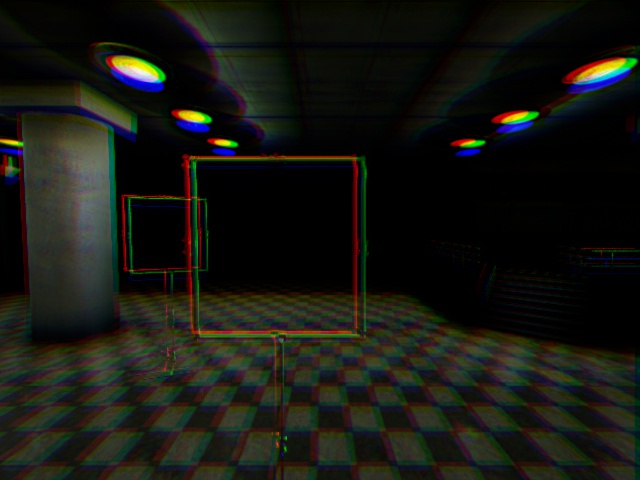
\includegraphics[width=\textwidth]{fig/gate_example_chromatic}
		\caption{Chromatic Aberration.} 		
		\label{fig:chromatic}
	\end{minipage}
	\begin{minipage}{0.33\textwidth}
		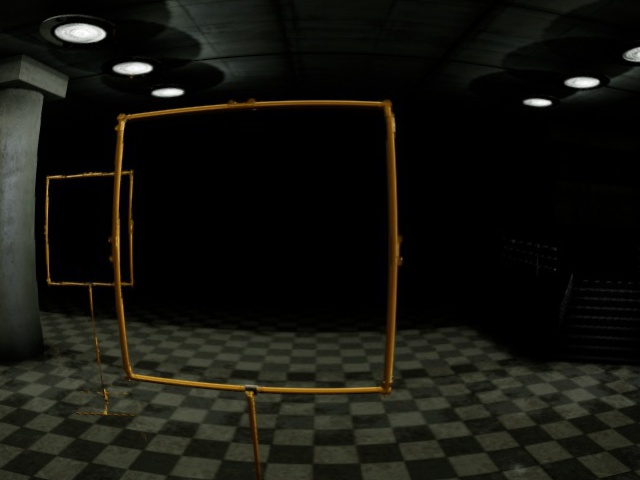
\includegraphics[width=\textwidth]{fig/gate_example_distorted}
		\caption{Lens Distortion. }		
		\label{fig:distortion}
	\end{minipage}
	
	\begin{minipage}{0.33\textwidth}
		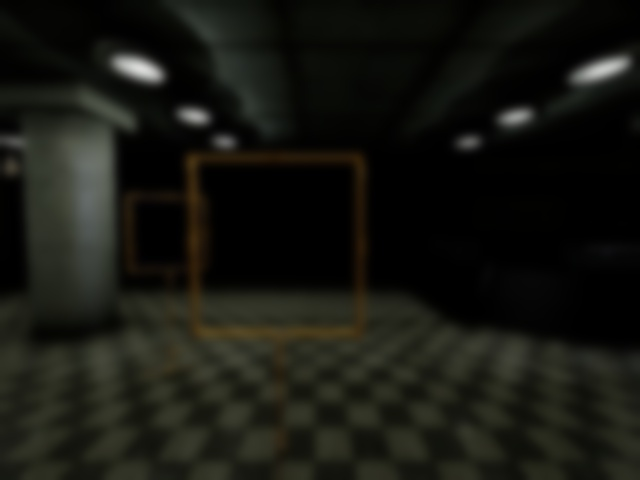
\includegraphics[width=\textwidth]{fig/gate_example_focusblur}
		\caption{Out-of-Focus blur.}
		\label{fig:focusblur}
	\end{minipage}
	\begin{minipage}{0.33\textwidth}
		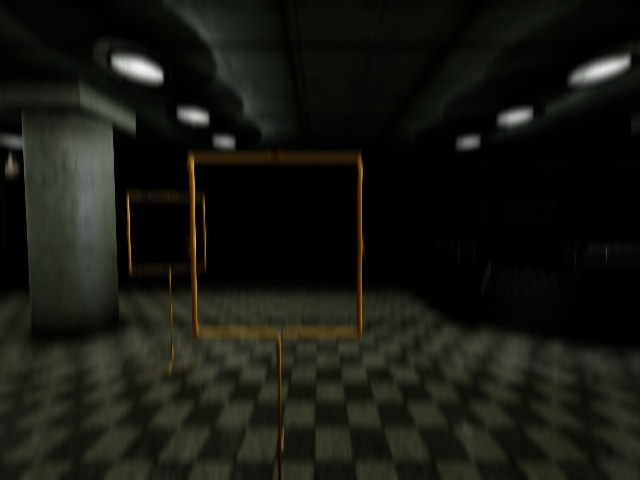
\includegraphics[width=\textwidth]{fig/gate_example_motionblur_v}
		\caption{Vertical Motion Blur.}
		\label{fig:motionblur}
	\end{minipage}
	\begin{minipage}{0.33\textwidth}
		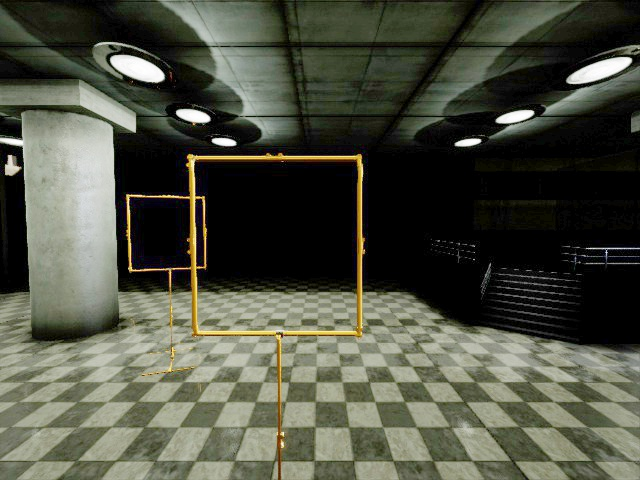
\includegraphics[width=\textwidth]{fig/gate_example_exposure}
		\caption{Exposure.}
		\label{fig:exposure}
	\end{minipage}
\end{figure}


\section{Object Detector}

This work uses a typical one-stage detector with anchor boxes as baseline, namely the \textit{YoloV3} detector with the \textit{TinyYoloV3} network. The fundamental concept of one-stage detectors with anchor boxes is illustrated in \Cref{sec:related}. In this section the implementation with the \textit{TinyYoloV3} network and its training goal are explained.

On a high level basis \textit{YoloV3} maps the input image to a predefined set of anchor boxes which are visualized in \Cref{sec:anchors}. The anchors have a predefined width $p_w$, height $p_h$ and are arranged in grids corresponding to the spatial resolution of the output layers. For objects of different scales different image features are relevant. Furthermore, for small objects a more fine grain resolution is required to sufficiently distinguish between multiple small objects close to each other. Therefore, \textit{YoloV3} uses two output grids $G=2$ output grids, with a grid of $S_1 =13$ for larger objects (red) and $S_2 = 26$ smaller objects (blue). 


For each box the network predicts an object probability $\hat o$ that classifies the class as object (1) or background (0). The original version of \textit{YoloV3} further distinguishes between object classes, however this work considers the single class case. There we remove this output node from the prediction. 

The predefined anchors only cover a subset of possible areas that can contain an object. Hence, \textit{YoloV3} also predicts how to adapt the anchor box to better fit the predicted object. These are  the bounding box center $b_x,b_y$ as well as its width $b_w$ and height $b_h$. 

In total this leads to 5 predicted parameters for each bounding box and thus to a mapping from the input image of 416x416x3 pixels to 12675 output nodes that predict 2535 boxes. In a last step boxes that contain the same class and have a high overlap are filtered such that only the boxes with the highest confidences remain.	

\subsection{Architecture}

This mapping is implemented with a \acp{CNN} as illustrated in  \Cref{fig:tinyyolov3_arch}. It contains 10 convolutional, 6 pooling and 1 unpooling layer(s). After each convolutional layer batch normalization normalizes the output in order to simplify the training process.
The input image with a resolution of 416x416x3 is processed by 5 layers that stepwise decrease the spatial resolution (max pooling) while increasing the width, leading to a intermediate volume of 26x26x512. This part can be seen as a common part that extracts features for objects at all scales. The architecture is a typical example of current \acp{CNN}. In the early layers the receptive field of the filters is small. Hence, the patterns that can be represented are not very complex and only a small amount of filters is used. As the network gets deeper more complex patterns can be present and more weights are required to encode these features. Hence, the width is increased. Research has shown that fixing kernels to a size of 3x3 and stacking them in deep layers is particularly efficient\todoref{vgg}. This can also be seen in the \textit{TinyYoloV3} architecture. 

Convolving the wide volume of deeper layers such as the 26x26x512  output of layer 5 with a 3x3 kernel requires many computations. Therefore a common technique is to first compress the volume by applying a 1x1 kernel intermediately. Such \textit{bottleneck} layers can be seen in layer 6-1 and 7-2.

From layer 5 the network splits to two branches responsible for smaller and larger objects. The lower branch extracts features for larger objects leading to a final grid of 13x13. The higher branch extracts features for smaller objects leading to a grid of 26x26. When Although not stated explicitly by the authors this is likely to compress the feature response of the previous layer and thus save computations.

In the final layer 15 output nodes are responsible to predict 3 bounding boxes for each grid cell. Thereby the nodes responsible for $\hat o$ have a sigmoid-activation such that the response gets squashed between 0 and 1 thus can be interpreted as a probability. Similarly the nodes responsible for $\hat x$ and $\hat y$ have a sigmoid activation such that the output can be interpreted as coordinate normalized to the image size. For the output nodes of $w$ and $h$ \textit{YoloV3} uses $e^x$-activation. This way the output is always larger than one while no adaption in bounding box width/height ($w=1$) corresponds to no activation. Furthermore, the network can predict a large range of scales in a small range of activation which aims to simplify the learning process.


\begin{figure}[hbtp]
	\centering
	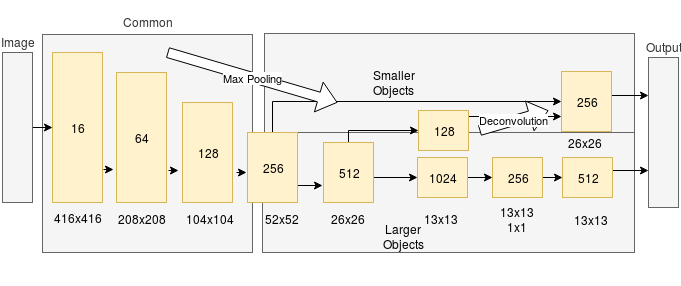
\includegraphics[width=0.8\textwidth]{fig/tinyyolov3_arch}
	\caption{The architecture of the baseline \textit{TinyYoloV3}. For each layer the amount of filters are displayed. The height of the boxes correspond to their spatial dimension. Arrows correspond to the forward pass in a network inference. In the common part the spatial resolution decreases each layer down to 26x26, while the width increases from 16 to 512. From layer 5 two branches focus on objects corresponding to different scales. }
	\label{fig:tinyyolov3_arch}
\end{figure}

	\subsection{Training Goal}

In order to train a \ac{CNN} to predict the desired properties a ground truth has to be defined for each of the 12675 output nodes. Subsequently the loss is formulated as derivable function and the \ac{CNN} can be trained with backpropagation.

Thereby it is desirable that a network output of zero corresponds to no network activation and henceforth to keep all predicted bounding boxes in the default shape. Therefore, \textit{YoloV3} encodes the ground true coordinates as follows:


\begin{equation}
\label{sec:encoding}
b_x = \sigma(\hat x_{i,j,k}) + g^x_{i,j}\quad
b_y = \sigma(\hat y_{i,j,k}) + g^y_{i,j}\quad
b_w = e^{\hat w_{i,j,k}} \cdot p^w_{i,j,k}\quad
b_h = e^{\hat h_{i,j,k}} \cdot p^h_{i,j,k}
\end{equation}

where $\hat{x}$,$\hat{y}$,$\hat w_{i,j,k}$ and $\hat h_{i,j,k}$ correspond to output nodes of anchor box at grid $i$, cell $j$, anchor $k$; $g^x_{i,j,k}$, $g^y_{i,j}$ is the top left coordinate of the respective grid cell; $\sigma$ is the sigmoid-function.

The question remains to which grid cell and anchor box a label is assigned to. Therefore the \ac{IoU} between every ground truth and anchor box is calculated and the grid with the highest value is assigned. If a ground truth box has very different coordinates than any possible anchor box, even the highest \ac{IoU} is comparatively low. Thus the network has to perform a very strong activation to predict such a label. In return the gradient will be high which can cause unstable updates. Therefore labels that have a lower \ac{IoU} than 0.5 are excluded. 

With the true label and the predicted label the training goal can be formulated. The loss needs to capture the localization and the classification goal. In a typical ground truth image only a small subset of anchors is assigned responsible to predict an object. All the other anchors see only background. Hence, there is a class imbalance between the "object" class and the "background" class. Treating both losses equally would lead the model to simply assign "background" for all anchors. The weight terms $\lambda_{obj}$ and $\lambda_{noobj}$ compensate for this class imbalance. Furthermore, $\lambda_{loc}$ trades-off the localization goal and the classification goal. The abstract training loss is summarized in: 

\begin{equation}
\mathcal{L} = \lambda_{loc}\mathcal{L}_{loc} + \lambda_{obj}\mathcal{L}_{obj} + \lambda_{noobj}\mathcal{L}_{noobj} + \lambda_{class}\mathcal{L}_{class}
\end{equation}
where $\mathcal{L}_{loc}$ is the loss for bounding box dimensions, $\mathcal{L}_{obj}$ the loss where a object is present, $\mathcal{L}_{noobj}$ the loss where there is no object. The weights are kept to the default value of $\lambda_{loc} = 5$,$\lambda_{obj} = 5$ and $\lambda_{noobj} = 0.5$.

The object loss quantifies a binary classification loss. Hence, it is the difference between a predicted probability $\hat o$ and an actual class label $c$. Where $o \in \{0,1\}$ and $\hat o \in (0,1)$. In order to learn such a goal it is desirable that the weights of the network get updated significantly when the difference between truth and prediction are high. However, when prediction and truth are already close to each other, the updates to the weights should be smaller otherwise the training might miss the optimal solution. A loss function that contains the desired properties and is used by \textit{YoloV3} is the logarithmic loss which can be formulated as follows:

\begin{equation}
\mathcal{L}_{log} = -(o_{ij}\log(\hat o_{ijk}) + (1 - o_{ij})\log(1 - \hat o_{ijk}))
\end{equation}

where $\hat o_{ij}$ is an output node with sigmoid activation assigned to anchor box $i$,$j$,$k$ and $ o_{ij}$ the ground truth label assigned to that box. The logarithmic loss is calculated for each output grid $G_i$, for each grid cell $S_j$ and each anchor box $B_k$. However, only the loss of the responsible anchor boxes are summed in the total loss calculation:

\begin{equation}
\mathcal{L}_{obj} = \sum_{i=0}^{G}\sum_{j=0}^{S_i^2}\sum_{k=0}^{B_i} \mathbb{1}_{ijk}^{obj}(-(c_{ijk}\log(\hat c_{ijk}) + (1 - c_{ijk})\log(1 - \hat c_{ijk})))
\end{equation}

Thereby the  binary variable $\mathbb{1}_{ijk}^{obj}$ is 1 if an object is present at anchor $i,j,k$. $\mathcal{L}_{obj}$ is defined vice versa but controlled by the $\mathbb{1}_{ijk}^{noobj}$ binary variable.

For the localization loss, similar to the classification loss, the weights should be updated significantly when the difference is high but less strongly when the difference is small. Furthermore, the loss should be invariant to direction. A loss that contains these properties is the squared distance between each bounding box parameter. However, the squared distance does not make a difference between large and small boxes. For example, a deviation of 5 px for a small ground truth box with a width of 1 is treated equally to a deviation from a ground truth box with width 100. Therefore \textit{YoloV3}, applies the square root on width and height to scale down very large box dimensions and thus balance the loss calculation. The localization loss is summarized in:

\begin{equation}
\mathcal{L}_{loc} = \sum_{i=0}^{G} \sum_{j=0}^{S_i^2}\sum_{k=0}^{B_i} \mathbb{1}_{ijk}^{obj}[(x_{ijk}-\hat{x}_{ijk})^2 + (y_{ijk}-\hat{y}_{ijk})^2  + (\sqrt{w_{ijk}}-\sqrt{\hat{w}_{ijk}})^2 +(\sqrt{h_{ijk}}-\sqrt{\hat{h}_{ijk}})^2 ]
\end{equation}
where $x_{ijk}$,$y_{ijk}$ are the ground truth center coordinates of anchor box $i,j,k$ and $w_{ijk}$,$h_{ijk}$ the corresponding width and height. $\hat x_{ijk}$,$\hat y_{ijk}, \hat w_{ijk}$,$\hat h_{ijk}$ are the predicted bounding box coordinates. 

The model is implemented using \textit{keras} with \textit{tensorflow} backend. 